\documentclass{article}
\usepackage[
				pdftex,
				colorlinks=true,
				bookmarksnumbered=true,
				bookmarksopen=true,
				bookmarksopenlevel=3,
				pdfstartview=FitP,
				urlcolor=blue,
			]{hyperref}
\pdfinfo{
			/Title(Esercitazione di Laboratorio: Circuiti con diodi)
			/Author(Coa Giulio, Licastro Dario, Montano Alessandra)
		}
\usepackage[italian]{babel}
\usepackage{geometry,titling,mdsymbol,stmaryrd,graphicx,subcaption,amsmath}
\graphicspath{{./Image/}}
\renewcommand\maketitlehooka{
								\null
								\mbox{}
								\vfill
							}
\renewcommand\maketitlehookd{
								\vfill
								\null
							}
\title{
		\begin{center}
			Esercitazione di Laboratorio:
		\end{center}
		\newline
		\begin{center}
			Circuiti con diodi
		\end{center}
	}
\author{
			Coa Giulio
			\and
			Licastro Dario
			\and
			Montano Alessandra
		}
\begin{document}
	%-----------------------------------------------------------------------------
	%  TITLE
	%-----------------------------------------------------------------------------
	\begin{titlingpage}
		\maketitle
	\end{titlingpage}
	\newpage
	%-----------------------------------------------------------------------------
	%  PURPOSE OF THE EXPERIENCE
	%-----------------------------------------------------------------------------
	\section{Scopo dell'esperienza}
		.
	%-----------------------------------------------------------------------------
	%  INSTRUMENTATION USED
	%-----------------------------------------------------------------------------
	\section{Strumentazione utilizzata}
		La strumentazione usata durante l'esercitazione è:
		\begin{center}
			\begin{tabular}{ |c|c|c| }
				\hline
				\multirow{\textbf{Strumento}}	 & \textbf{Marca e Modello} & \textbf{Caratteristiche} \\
				\hline
				\multirow{Multimetro}			 & Agilent 34401A			& \\
				\multirow{Oscilloscopio}		 & Rigol DS1054Z			& 4 canali, \\
												 &							& $ B = 50 \, \mathrm{MHz} $, \\
												 &							& $ f_{\mathrm{c}} = 1 \, \mathrm{G\frac{Sa}{s}} $, \\
												 &							& $ R_{\mathrm{i}} = 1 \, \mathrm{M\Omega} $, \\
												 &							& $ C_{\mathrm{i}} = 13 \, \mathrm{pF} $, \\
												 &							& $ 12 \, \mathrm{Mbps} $ di profondità di memoria \\
				\multirow{Generatore di segnali} & Rigol DG1022				& 2 canali, \\
												 &							& $ f_{\mathrm{uscita}} = 20 \, \mathrm{MHz} $, \\
												 &							& $ Z_{\mathrm{uscita}} = 50 \, \mathrm{\Omega} $ \\
				\multirow{Sonda}				 & Rigol PVP215				& $ B = 35 \, \mathrm{MHz} $, \\
												 &							& $ V_{\mathrm{nominale}} = 300 \, \mathrm{V} $, \\
												 &							& $ L_{\mathrm{cavo}} = 1.2 \, \mathrm{m} $, \\
												 &							& $ R_{\mathrm{s}} = 1 \, \mathrm{M\Omega} $, \\
												 &							& Intervallo di compensazione: $ 10 \div 25 \, \mathrm{pF} $ \\
				\multirow{Cavi coassiali}		 &							& Capacità dell'ordine dei $ 80 \div 100 \, \mathrm{p\frac{F}{m}} $ \\
				\multirow{Connettori}			 &							& \\
				\multirow{Breadboard}			 &							& \\
				\multirow{Diodo zener}			 &							& \\
				\multirow{Diodo}				 &							& \\
				\multirow{Condensatori}			 &							& $ C_{1} = 10 \, \mathrm{nF} $, \\
												 &							& $ C_{2} = 100 \, \mathrm{nF} $, \\
												 &							& $ C_{3} = 1 \, \mathrm{\mu F} $ \\
				\hline
			\end{tabular}
		\end{center}
	%-----------------------------------------------------------------------------
	%  THEORETICAL PREMISES
	%-----------------------------------------------------------------------------
	\section{Premesse teoriche}
		\subsection{Incertezza sulla misura dell'oscilloscopio}
			La misura del valore di un segnale tramite l’oscilloscopio (sia esso l'ampiezza, la frequenza, il periodo, etc.) presenta un'incertezza che dipende, principalmente, da due fattori:
			\begin{itemize}
				\item l’incertezza strumentale introdotta dall’oscilloscopio (ricavabile dal manuale).
				\item l’incertezza di lettura dovuta all’errore del posizionamento dei cursori.
			\end{itemize}
			Quest’ultima incertezza deriva dal fatto che il segnale visualizzato non ha uno spessore nullo sullo schermo.
		\subsection{Sonda}
			La sonda è un particolare cavo coassiale che presenta un'estremità capace di effettuare delle misurazioni.
			\newline
			Quando si usano dei classici cavi coassiali BNC-BNC al fine di collegare il circuito, su cui effettuare le misure, all'oscilloscopio, si sta inserendo in parallelo al circuito un condensatore di capacità ($ C_{\mathrm{c}} $) pari a quella del cavo.
			\begin{figure}[h!]
				\centering
				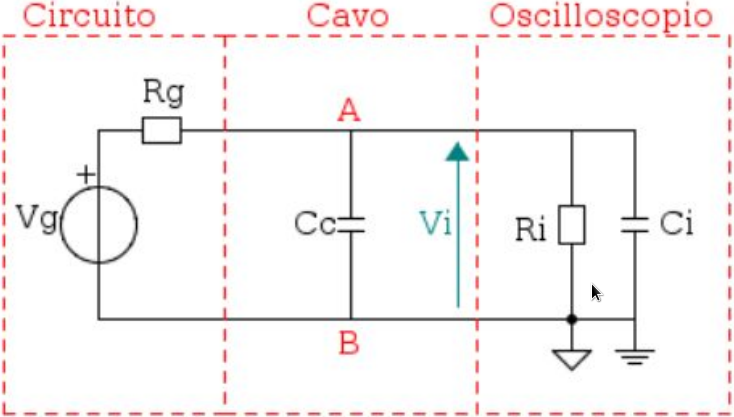
\includegraphics[scale=0.4]{theveninCavoDSO}
				\caption{Circuito analizzato collegato all'oscilloscopio tramite un cavo coassiale BNC-BNC.}
				\label{fig:theveninCavoDSO}
			\end{figure}
			\newpage
			In questo caso, l’oscilloscopio si comporta, in ingresso, come un filtro passa-basso con una frequenza di taglio ($ f = \frac{1}{2\pi R_{i} (C_{s} + C_{i})} $). L'uso di una sonda per misurare delle grandezze in un circuito, si può vedere come l'inserimento di un condensatore in serie al circuito.
			\begin{figure}[h!]
				\centering
				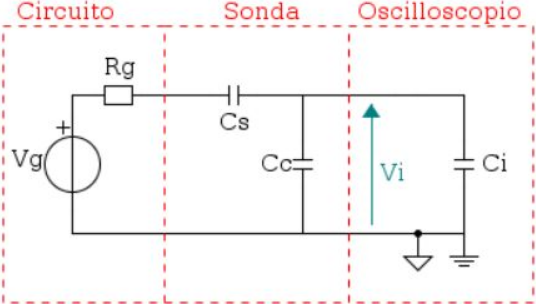
\includegraphics[scale=0.4]{theveninSondaDSOCircuito}
				\caption{Circuito analizzato collegato all'oscilloscopio tramite una sonda.}
				\label{fig:theveninSondaDSOCircuito}
			\end{figure}
			\newline
			L'introduzione di questo condensatore comporta un calo della capacità equivalenti vista all'ingresso del circuito ($ \mathrm{\frac{C_{s} (C_{c} + C_{i})}{C_{s} + C_{c} + C_{i}} \ll C_{c} + C_{i}} $), ovvero una riduzione della frequenza del polo ($ f_{\mathrm{polo}} = \frac{1}{2\pi R_{i} (C_{s} + C_{i})} $); ciò porta ad una perdita d'informazioni in bassa frequenza.
			\newline
			Al fine di evitare tale perdita d'informazioni, si pone, in parallelo al condensatore, una resistenza.
			\begin{figure}[h!]
				\centering
				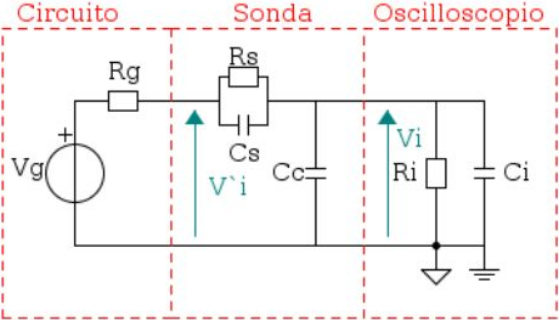
\includegraphics[scale=0.4]{theveninSondaDSOResistenza}
				\caption{Circuito analizzato collegato all'oscilloscopio tramite una sonda.}
				\label{fig:theveninSondaDSOResistenza}
			\end{figure}
			\newline
			Tale resistenza comporta la presenza di uno zero, oltre al polo precedentemente detto.
			\begin{figure}[h!]
				\centering
				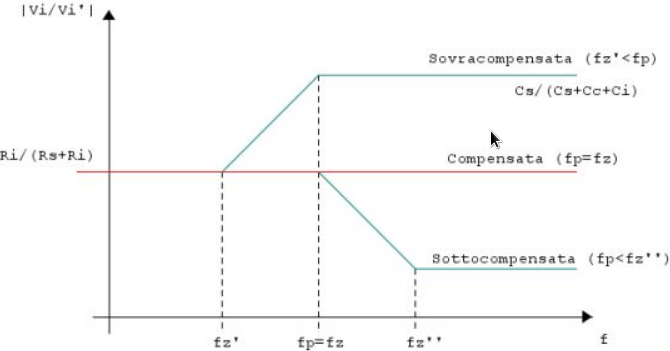
\includegraphics[scale=0.4]{sondaBode}
				\caption{Diagramma di Bode della funzione di trasferimento del circuito.}
				\label{fig:sondaBode}
			\end{figure}
			\newpage
			A seconda dell'elevata o della bassa compensazione della sonda, il segnale sarà distorto verso l'alto o verso il basso.
			\begin{figure}[h!]
				\centering
				\begin{subfigure}{0.4\textwidth}
					\centering
					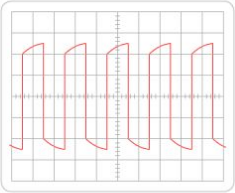
\includegraphics[scale=0.5]{sondaSegnaleSottocompensato}
					\caption{Sonda sottocompensata.}
				\end{subfigure}
				\begin{subfigure}{0.4\textwidth}
					\centering
					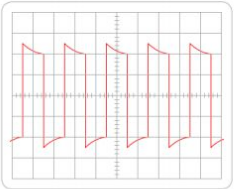
\includegraphics[scale=0.5]{sondaSegnaleSovracompensato}
					\caption{Sonda sovracompensata.}
				\end{subfigure}
				\caption{Visualizzazione del segnale al variare della compensazione della sonda.}
				\label{fig:sondaSegnaleNonCompensato}
			\end{figure}
			\newline
			La sonda risulta compensata quando la frequenza del polo coincide con la frequenza dello zero; ciò avviene quando $ R_{\mathrm{s}} C_{\mathrm{s}} = R_{\mathrm{i}} (C_{\mathrm{c}} + C_{\mathrm{i}})} $. La sonda presenta un opportuno trimmer che influenza il valore di $ R_{\mathrm{s}} $ e permette la compensazione. Al fine di verificare se la sonda è compensata si esegue un confronto con un segnale noto.
			\begin{figure}[h!]
				\centering
				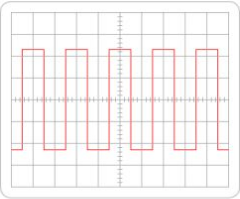
\includegraphics[scale=0.5]{sondaSegnaleCompensato}
				\caption{Sonda compensata.}
				\label{fig:sondaSegnaleCompensato}
			\end{figure}
		\subsection{Other}
			.
	%-----------------------------------------------------------------------------
	%  LABORATORY EXPERIENCE
	%-----------------------------------------------------------------------------
	\section{Esperienza in laboratorio}
		\subsection{Caratteristiche statiche}
			.
		\subsection{Raddrizzatore a semplice semionda}
			.
		\subsection{Rivelatore di picco}
			.
		\subsection{Circuito per la protezione da scariche elettrostatiche}
			.
	%-----------------------------------------------------------------------------
	%  RESULTS
	%-----------------------------------------------------------------------------
	\section{Risultati}
		\subsection{Caratteristiche statiche}
			.
		\subsection{Raddrizzatore a semplice semionda}
			.
		\subsection{Rivelatore di picco}
			.
		\subsection{Circuito per la protezione da scariche elettrostatiche}
			.
	%-----------------------------------------------------------------------------
	%  CONCLUSION
	%-----------------------------------------------------------------------------
	\section{Conclusioni}
		\subsection{Caratteristiche statiche}
			.
		\subsection{Raddrizzatore a semplice semionda}
			.
		\subsection{Rivelatore di picco}
			.
		\subsection{Circuito per la protezione da scariche elettrostatiche}
			.
\end{document}